\documentclass[11pt]{beamer}
\usetheme{default} 

\setbeamertemplate{navigation symbols}{} %gets rid of navigation symbols
\setbeamertemplate{footline}{} %gets rid of bottom navigation bars
\setbeamertemplate{footline}[page number]{} %use this for page numbers

\setbeamertemplate{footline}{%
  \raisebox{5pt}{\makebox[\paperwidth]{\hfill\makebox[10pt]{\scriptsize\insertframenumber~~}}}}

\setbeamertemplate{itemize items}[circle] %round bullet points
\setlength\parskip{10pt} % white space between paragraphs

\usepackage{wrapfig}
\usepackage{subfig}
\usepackage{setspace}
\usepackage{enumerate}
\usepackage{graphicx}
\usepackage{amsmath}
\usepackage{amsfonts}
\usepackage{amssymb}
\usepackage{amsthm}
\usepackage[UKenglish]{isodate}
\usepackage{tikz}
\usepackage{pgfplots}
\usepackage{natbib}
\usepackage{hyperref}
\hypersetup{
    colorlinks=true, 
    urlcolor=blue
}
\def\checkmark{\tikz\fill[scale=0.4](0,.35) -- (.25,0) -- (1,.7) -- (.25,.15) -- cycle;} 

% allow drawing arrows
\usetikzlibrary{arrows}
\tikzstyle{arrow}=[draw, -latex] 

% bracketing shortcuts
\newcommand{\paren}[1]{\left(#1\right)}
\newcommand{\sqbracket}[1]{\left[#1\right]}
\newcommand{\cbracket}[1]{\left\{#1\right\}}
\newcommand{\abs}[1]{\left\lvert#1\right\rvert}
\newcommand{\norm}[1]{\left\lVert#1\right\rVert}
% set up the argmin operator, argmax
\DeclareMathOperator*{\argmin}{arg\,min}
\DeclareMathOperator*{\argmax}{arg\,max}

\newcommand{\myframe}[1]{\begin{frame} \frametitle{#1}}

% New itemize environment, with spaces
\newenvironment{spaceitemize}
{ \begin{itemize}
    \setlength{\itemsep}{10pt}
    \setlength{\parskip}{0pt}
    \setlength{\parsep}{0pt}     }
{ \end{itemize}                  } 


% the preamble
\title{Day 3, Session 1: R basics}
\author{Jessica Williams-Nguyen and Brian D. Williamson}
\institute{EPI/BIOST Bootcamp 2017}
\date{26 September 2017}

% Start the document
\begin{document}
% The title page
\begin{frame}
\titlepage
\end{frame}

% R intro
\section{R and RStudio}
\myframe{Command line R}
The most basic form of R is from the command line (Terminal in Mac/Linux, Command Prompt in Windows). 

After installing R, typing R in the command line will open an R session:
\begin{center}
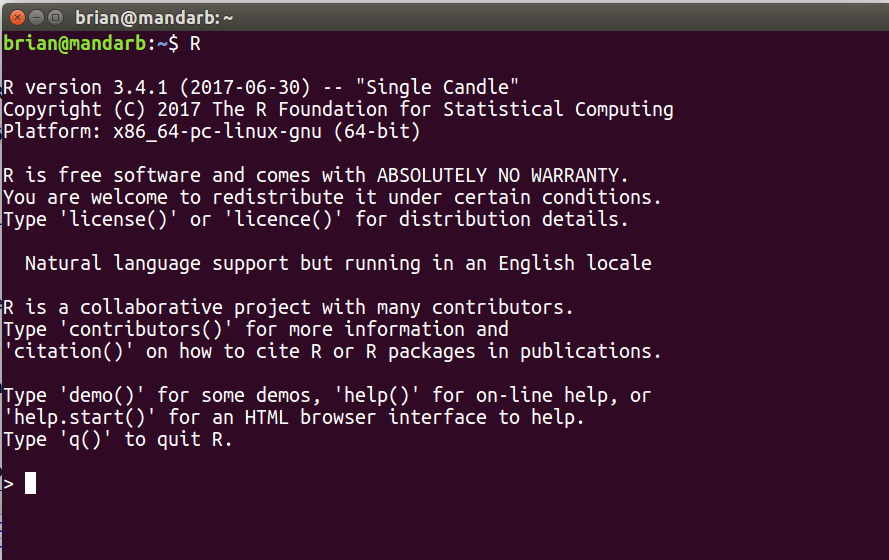
\includegraphics[width = .6\textwidth]{figs/command_line_r.png}
\end{center}

The text gives you the version number (here, 3.4.1) and some other (not necessary for our purposes) information. 
\end{frame}

\myframe{Command line R}
You also get a prompt, the \texttt{>}, where you can enter commands. 

When you first open R, you have a limited number of functions available for use. These include things like \texttt{mean()}, \texttt{median()}, and \texttt{read.table()}. 

The command line version of R is most useful (in my experience) for computing-intensive tasks. Data analyses are best done in RStudio.
\end{frame}

\myframe{RStudio}
When you first open RStudio, you are met with a blank set of four \textcolor{blue}{panes}:
\begin{center}
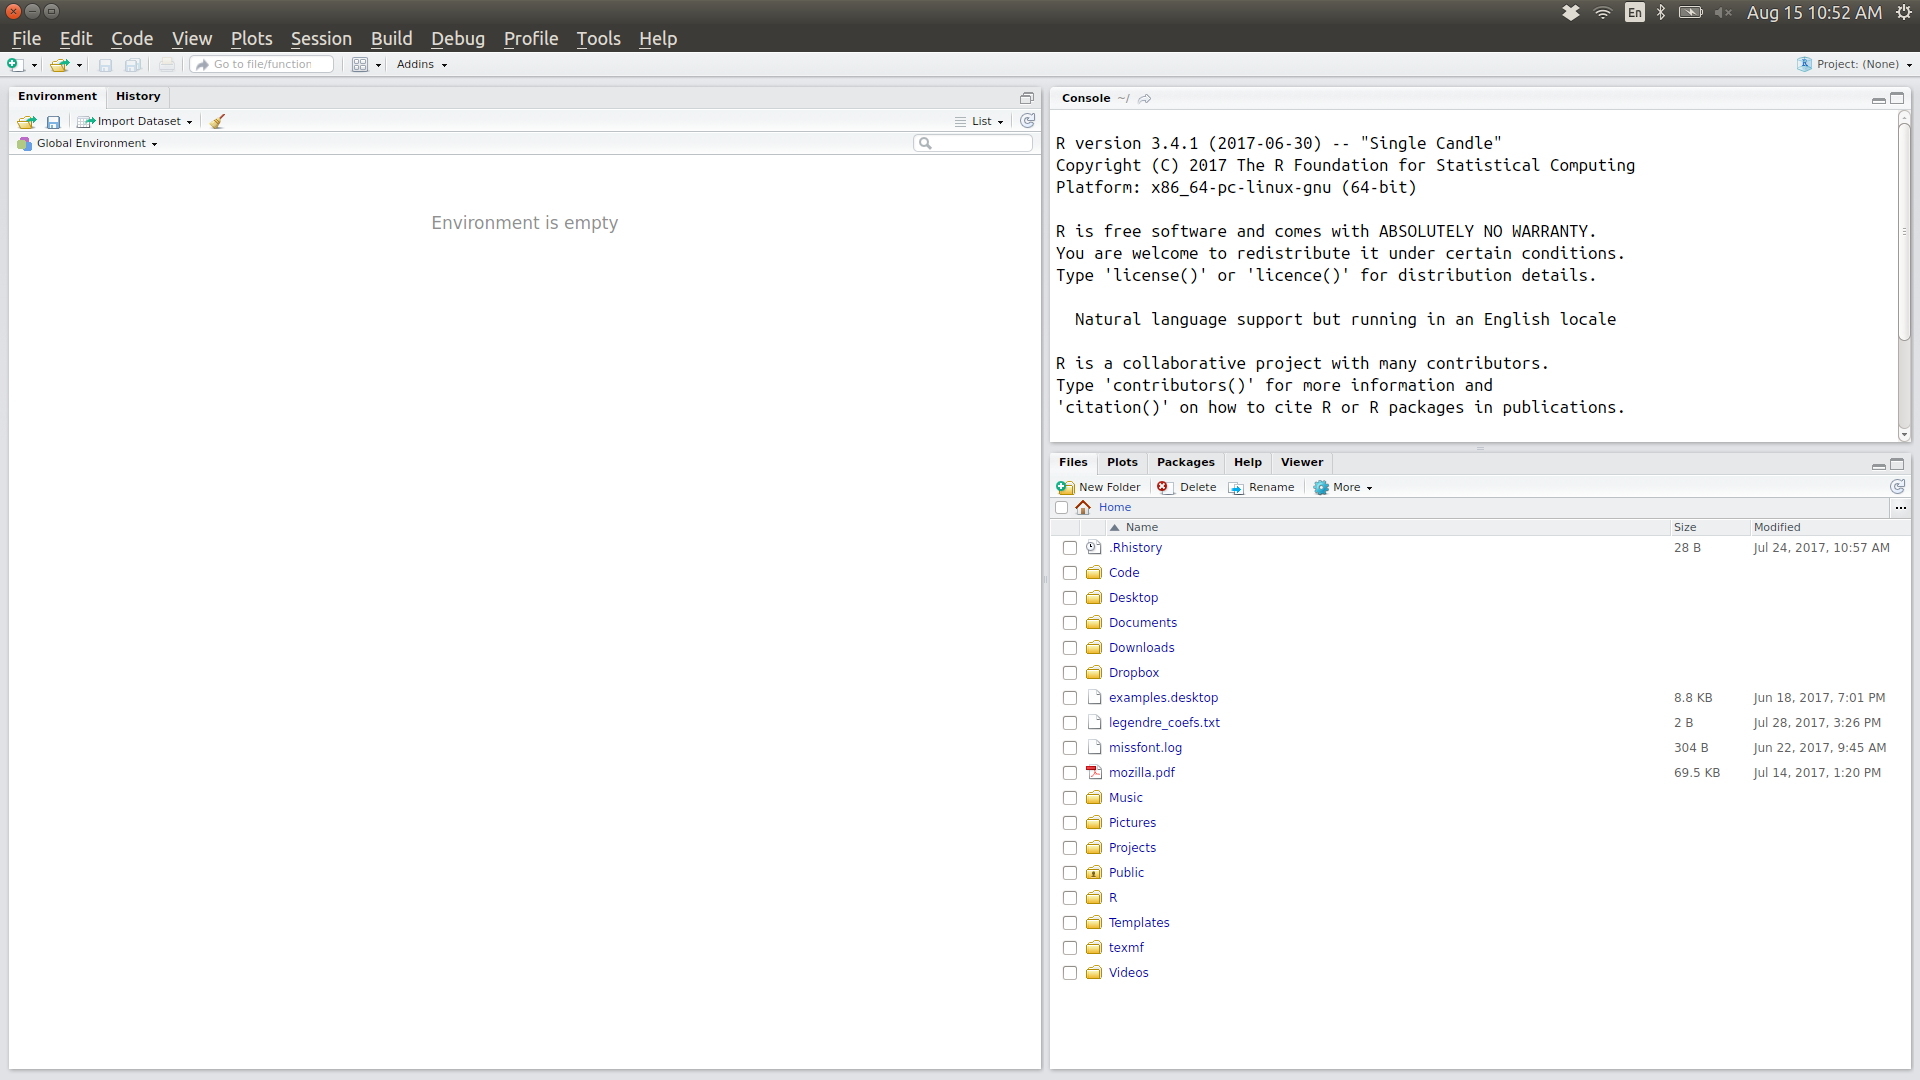
\includegraphics[width = 0.8\textwidth]{figs/rstudio.png}
\end{center}
\end{frame}

\myframe{RStudio}
You can edit pane layout under \texttt{Tools > Global Options > Pane Layout}. My preference is to have the \textcolor{blue}{source} in the upper left, \textcolor{green}{console} in the upper right, \textcolor{cyan}{environment} in the lower left, and \textcolor{purple}{viewer} in the lower right.

You'll notice that on the previous slide, there were only three panes visible: since we haven't opened or created any files to edit, the \textcolor{blue}{source} pane is not currently open.
\end{frame}

\myframe{RStudio: the console}
Is it a coincidence that the screenshot has exactly the same text as we saw on the command line? No! 

The \textcolor{green}{console} performs identically to the command line. Any commands that we wish to enter go through the console, and any results that are output by these commands will appear in the console. 

\end{frame}

\begin{frame}[fragile]
\frametitle{Example: the console}
Typing \texttt{47} at the \texttt{>} symbol (from now on, called the execution line) and hitting \texttt{Enter} on the keyboard yields the following:
\begin{verbatim}
> 47
[1] 47
\end{verbatim}

Since R is a \textcolor{blue}{functional} programming language, typing \texttt{47} and hitting \texttt{Enter} is the same thing as using the \texttt{print()} function:
\begin{verbatim}
> print(47)
[1] 47
\end{verbatim}

The output is displayed as a \textcolor{green}{vector}, one of the fundamental \textcolor{cyan}{data structures} in R. The \texttt{[1]} helps to tell which element of the vector we are looking at (which is most useful if the vector spans multiple lines in the console).
\end{frame}

\myframe{Example: heights and weights}
The console is the workhorse of RStudio. If we wanted, we could work exclusively here, but then reproducibility is difficult...

Let's say we have data on the height and weight of five (imaginary) individuals. A simple way of reading the data into R is by creating two \textcolor{blue}{objects}, \texttt{ht} and \texttt{wt}, and assigning the numerical values that we have collected for each individual; in the console, type
\begin{enumerate}
\item \texttt{ht <- c(72,65,84,73,68)}, followed by hitting the \texttt{Enter} key, (creates the \texttt{ht} object)
\item \texttt{wt <- c(165,120,210,180,125)}, followed by hitting the \texttt{Enter} key (creates the \texttt{wt} object)
\end{enumerate}

Each of these commands assigns a \textcolor{green}{value} to an \textcolor{blue}{object}, using the special \texttt{<-} command. \textcolor{green}{Values} go on the right-hand side, and \textcolor{blue}{objects} go on the left.
\end{frame}

\myframe{Example: heights and weights}
Both \texttt{ht} and \texttt{wt} are also vectors! We create vectors using the \texttt{c()} function, which concatenates scalars (single numbers, or single strings like \texttt{"Hello"}) into vectors.

In words, \texttt{ht <- c(72,65,84,73,68)} means: concatenate the numbers 72, 65, 84, 73, and 68 into a vector, and assign that vector to a variable (or object) called \texttt{ht}.

Typing these commands into the console allows us to manipulate both \texttt{ht} and \texttt{wt}; in particular, they can be used as arguments into many R functions.
\end{frame}

\myframe{Example: heights and weights}
However, these objects are part of the \textcolor{red}{current} R environment: this means that we can only use them while the current session of R is open. If we exit RStudio, we will have to re-enter the two lines defining both \texttt{ht} and \texttt{wt}.

For more complicated analyses, this can lead to a lot of confusion. Also, just typing in the console can lead us to forget what steps we took to get a certain figure or table.

Organizing commands into \textcolor{blue}{scripts} allows us to save exactly what we did during a given data analysis, which makes reproducible research easy. This helps both your future self and your collaborators, so that you can share what you did!
\end{frame}


\myframe{RStudio: the text editor (``Source'')}
The text editor (which RStudio calls the \textcolor{blue}{source}) is the second most powerful part of the IDE. This allows us to edit and save files, and to run commands directly from the text file into the console.

To create a new R script, either type \texttt{Ctrl+Shift+N} or go to \texttt{File > New > R script}. There are many other options here (most notably R markdown, which we won't cover but is incredibly useful). This brings up the source pane.

At the top of the source pane are a set of buttons (with associated keyboard shortcuts) that will save the current file, run sections of code, or run the entire document. 
\end{frame}

\begin{frame}[fragile]
\frametitle{R scripts}
R scripts are collections of R commands and comments. These are run in the console to manipulate objects and produce output.

To create a comment, type a \texttt{\#} symbol. Anything on a line following a \texttt{\#} will not be run by R.

I like to include a preamble in all of my R scripts, which gives me information on when I created the file, what it does, whether or not it takes any input or produces output, and what I have changed since I started. Here is a sample:
\fontsize{7pt}{7.2}\selectfont
\begin{verbatim}
##############################################################################################
##
## FILE: <insert file name here>.R
##
## CREATED: <insert date here> by <your name here>
##
## PURPOSE: <Give a brief description of what the code in this file is supposed to do>
##
## INPUTS: <What inputs? Where does the data come from?>
##
## OUTPUTS: <What outputs? Plot/table names and locations>
##
## UPDATES:
## DDMMYY INIT COMMENTS
## ------ ---- --------
## <date> <inits> <What did you change?>
##############################################################################################
\end{verbatim}
\end{frame}

\begin{frame}[fragile]
\frametitle{Example: heights and weights}
We can now enter 
\begin{verbatim}
ht <- c(72,65,84,73,68)
wt <- c(165,120,210,180,125)
\end{verbatim}
into a new R script. Saving this as \texttt{ht\_wt\_analysis.R} is a start to analyzing these data! The script now looks like:
\tiny
\begin{verbatim}
##############################################################################################
##
## FILE: ht_wt_analysis.R
##
## CREATED: 15 August 2017 by Brian Williamson
##
## PURPOSE: Teach some R basics using height and weight data on 5 imaginary individuals
##
## INPUTS: None
##
## OUTPUTS: None
##
## UPDATES:
## DDMMYY INIT COMMENTS
## ------ ---- --------
##############################################################################################

ht <- c(72,65,84,73,68)
wt <- c(165,120,210,180,125)
\end{verbatim}
\end{frame}

\myframe{RStudio: environment, file history, etc.}

\end{frame}

\myframe{RStudio: files, plot viewer, packages, help}

\end{frame}

\section{Introduction}
\myframe{Functions}

\end{frame}

\myframe{Objects}

\end{frame}

% Accessing and manipulating data
\section{Accessing and manipulating data}
\myframe{Loading data}

\end{frame}

\myframe{Saving data}

\end{frame}

\myframe{Manipulating data}

\end{frame}

\section{R packages}
\myframe{R packages}

\end{frame}

\end{document}